
%(BEGIN_QUESTION)
% Copyright 2011, Tony R. Kuphaldt, released under the Creative Commons Attribution License (v 1.0)
% This means you may do almost anything with this work of mine, so long as you give me proper credit

Examine this function block diagram for a control strategy:

$$\includegraphics[width=15.5cm]{i03280x01.eps}$$

Explain what sort of control strategy this is, based on what you can discern from this function block diagram.  Be as specific as you can in your answer!

\vfil 

\underbar{file i03280}
\eject
%(END_QUESTION)





%(BEGIN_ANSWER)

This is a graded question -- no answers or hints given!

%(END_ANSWER)





%(BEGIN_NOTES)

This is a {\it feedforward} control strategy, where one of three temperature transmitter inputs is selected to be the feedforward variable, and where flow is the feedback process variable.  

\vskip 10pt

The entire control system is implemented using FOUNDATION Fieldbus instruments, as indicated by the instrument tag names beneath each function block.

%INDEX% DCS, programming: function block program

%(END_NOTES)

